%%%%%%%%%%%%%%%%%%%%%%%%%%%%%%%%%%%%%%%%%
% Jacobs Landscape Poster
% LaTeX Template
% Version 1.0 (29/03/13)
%
% Created by:
% Computational Physics and Biophysics Group, Jacobs University
% https://teamwork.jacobs-university.de:8443/confluence/display/CoPandBiG/LaTeX+Poster
% 
% Further modified by:
% Nathaniel Johnston (nathaniel@njohnston.ca)
%
% This template has been downloaded from:
% http://www.LaTeXTemplates.com
%
% License:
% CC BY-NC-SA 3.0 (http://creativecommons.org/licenses/by-nc-sa/3.0/)
%
%%%%%%%%%%%%%%%%%%%%%%%%%%%%%%%%%%%%%%%%%

%----------------------------------------------------------------------------------------
%	PACKAGES AND OTHER DOCUMENT CONFIGURATIONS
%----------------------------------------------------------------------------------------

\documentclass[final]{beamer}

\usepackage{tikz}
%\usepackage{tikz}
\usepackage{graphicx}
\usepackage[scale=1.24]{beamerposter} % Use the beamerposter package for laying out the poster

\usetheme{confposter} % Use the confposter theme supplied with this template

\setbeamercolor{block title}{fg=ngreen,bg=white} % Colors of the block titles
\setbeamercolor{block body}{fg=black,bg=white} % Colors of the body of blocks
\setbeamercolor{block alerted title}{fg=white,bg=dblue!70} % Colors of the highlighted block titles
\setbeamercolor{block alerted body}{fg=black,bg=dblue!10} % Colors of the body of highlighted blocks
% Many more colors are available for use in beamerthemeconfposter.sty

%-----------------------------------------------------------
% Define the column widths and overall poster size
% To set effective sepwid, onecolwid and twocolwid values, first choose how many columns you want and how much separation you want between columns
% In this template, the separation width chosen is 0.024 of the paper width and a 4-column layout
% onecolwid should therefore be (1-(# of columns+1)*sepwid)/# of columns e.g. (1-(4+1)*0.024)/4 = 0.22
% Set twocolwid to be (2*onecolwid)+sepwid = 0.464
% Set threecolwid to be (3*onecolwid)+2*sepwid = 0.708

\newlength{\sepwid}
\newlength{\onecolwid}
\newlength{\twocolwid}
\newlength{\threecolwid}
\newlength{\leftcolwid}
\newlength{\midcolwid}
\newlength{\rightcolwid}
\setlength{\paperwidth}{48in} % A0 width: 46.8in
\setlength{\paperheight}{36in} % A0 height: 33.1in
\setlength{\sepwid}{0.02\paperwidth} % Separation width (white space) between columns
\setlength{\leftcolwid}{0.22\paperwidth} 
\setlength{\midcolwid}{0.35\paperwidth} 
\setlength{\rightcolwid}{0.35\paperwidth} 
\setlength{\onecolwid}{0.22\paperwidth} % Width of one column
\setlength{\twocolwid}{0.464\paperwidth} % Width of two columns
\setlength{\threecolwid}{0.708\paperwidth} % Width of three columns
\setlength{\topmargin}{-0.5in} % Reduce the top margin size
%-----------------------------------------------------------

\usepackage{graphicx}  % Required for including images

\usepackage{booktabs} % Top and bottom rules for tables
\usepackage{mathtools}
\usepackage{exscale} % otherwise \sum etc are messed up
\usepackage{tcolorbox}
\usepackage{caption}
\setbeamertemplate{caption}[numbered]
\include{poster_defs}
\definecolor{mydarkgreen}{RGB}{10,100,30}
%\include{figure_and_table}
%----------------------------------------------------------------------------------------
%	TITLE SECTION 
%----------------------------------------------------------------------------------------
\title{\LARGE Contextualized Sequence Likelihood: Enhanced Confidence Scores for Natural Language Generation} % Poster title

\author[zhenlin4@illinois.edu]{Zhen Lin$^1$ \hspace{4cm} Shubhendu Trivedi \hspace{4cm} Jimeng Sun$^{1,2}$}
\institute[UIUC]
{\hspace{4cm} $^1$ University of Illinois at Urbana-Champaign, $^2$ Carle Illinois College of Medicine}


%----------------------------------------------------------------------------------------

\begin{document}

%-----------LOGO ADDED TO NORTH EAST----------------%
\addtobeamertemplate{headline}{} 
{\begin{tikzpicture}[remember picture, overlay]
     \node [anchor=north east, inner sep=9cm]  at (current page.north east)
     {
\includegraphics[height=3.5cm]{poster_resources/illinois_logo.png}};
  \end{tikzpicture}}
%-------END LOGO ADDED TO NORTH EAST----------------%

%-----------LOGO ADDED TO NORTH WEST----------------%
\addtobeamertemplate{headline}{} 
{\begin{tikzpicture}[remember picture, overlay]
     \node [anchor=north west, inner sep=7.5cm] (node_1) at (current page.north west)
     {
\includegraphics[height=6cm]{poster_resources/github_QR.png}
     
\includegraphics[height=6cm]{poster_resources/sunlab.png}};
  % Add "code" text under the QR.png
  \node [font=\Large,xshift=5cm] at (node_1.west) {github:};
  \end{tikzpicture}}
 %-------END LOGO ADDED TO NORTH WEST----------------%

\addtobeamertemplate{block end}{}{\vspace*{2ex}} % White space under blocks
\addtobeamertemplate{block alerted end}{}{\vspace*{2ex}} % White space under highlighted (alert) blocks

\setlength{\belowcaptionskip}{2ex} % White space under figures
\setlength\belowdisplayshortskip{2ex} % White space under equations

\begin{frame}[containsverbatim,t] % The whole poster is enclosed in one beamer frame

\begin{columns}[t] % The whole poster consists of three major columns, the second of which is split into two columns twice - the [t] option aligns each column's content to the top

\begin{column}{\sepwid}\end{column} % Empty spacer column

\begin{column}{\leftcolwid} % The first column

%----------------------------------------------------------------------------------------
%	OBJECTIVES
%----------------------------------------------------------------------------------------

\begin{alertblock}{Highlights}

\begin{itemize}
\item Contextualized Sequence Likelihood (\methodname) improves the widely used sequence likelihood, by attending to the important tokens.

\item \methodname can serve as a quality metric for model generations in tasks like selective generation, or to improve other uncertainty quantification methods.

\item \methodname doesn't require additional model training, and has little-to-none overhead.
\end{itemize}

\end{alertblock}

%----------------------------------------------------------------------------------------
%	INTRODUCTION
%----------------------------------------------------------------------------------------
\begin{block}{\color{mydarkgreen}{Background: Sequence Likelihood}}
\begin{itemize}

\item The most commonly used confidence score function (likelihood of the generated sequenc, and the normalized version):

\begin{align}
    \Conf_{\baselineNLL} &= \sum_{i=1}^n l_i = \log{\prod_{i=1}^n \hat{p}(s_i|\predSeq_{<i},x)}\label{eq:confll}\\
    \text{C}_{\baselineNLLNorm} &= \frac{1}{n} \sum_{i=1}^n l_i \label{eq:confll:norm}.
\end{align}

\item 
Generally, higher $\Conf_{\baselineNLL}$ means higher confidence.

\item 
Sequence likelihood, however, conflates semantic and syntactic components.\\

\end{itemize}
\textbf{Examples:}
\begin{figure}[ht]
\begin{minipage}{0.5\textwidth}
{\small
\begin{align*}
\textbf{Q: } &\text{\textbf{Which country} won the World Cup in 2022?}\\
\textbf{A: } &\text{Messi won in the 2022 World Cup.}\\
& \textit{Incorrect answer;}\\
& \textit{High likelihood}\\\\
\textbf{Q: } &\text{\textbf{When} did Messi win the World Cup?}\\
\textbf{A: } &\text{Messi emerged victorious in the 2022 World Cup.}\\
& \textit{Correct answer;}\\
& \textit{Low likelihood due to the awkward wording}
\end{align*}
}
\end{minipage}
\end{figure}

\end{block}

\begin{block}{\color{mydarkgreen}{Contextualized Sequence Likelihood}}
\textbf{Idea:} Use appropriate attention values to overweight important tokens.
\begin{align}
    \ConfMethod = 
    \sum_{i=1}^n {{\color{red}w_i}} l_i 
    \text{ where } & w_i = \frac{a_{i}}{\sum_{i'=1}^n a_{i'}} \label{eq:main}
\end{align}
\end{block}
\end{column} % End of the first column

\begin{column}{\sepwid}\end{column} % Empty spacer column

\begin{column}{\midcolwid} % Begin a column which is two columns wide (column 2)

%\begin{columns}[t,totalwidth=\twocolwid] % Split up the two columns wide column

\begin{column}{\midcolwid}\vspace{-.6in} % The first column within column 2 (column 2.1)

%----------------------------------------------------------------------------------------
%	KDE
%----------------------------------------------------------------------------------------

\begin{block}{\color{mydarkgreen}{Step 1: Attention-Eliciting Prompt}}

To systematically identify the most relevant tokens, we first use a prompt to elicit the LM's attention on its own response $\predSeq$.

\begin{figure}[ht]
\begin{lstlisting}[basicstyle=\footnotesize\ttfamily]
Read the following question with optional context and decide if the answer correctly answers the question. Focus on the answer, and reply Y or N.
...
Context: Harry is a good witcher.
Question: How old is Harry?
Answer: Harry practices witchcraft.
 Decision: N. (The answer does not mention Harry's age.)
...
[$optional_context]
Question: [$question]
Answer: [$response]
 Decision: 
\end{lstlisting}
\end{figure}


% Assuming the $\predSeq_i$ becomes the $i'$-th token in the attention-eliciting prompt, the new confidence score could be written as:
% \begin{align}
%     \ConfMethod = \sum_{i=1}^n w_i l_i 
%     \text{ where } & w_i = \frac{a_{i}}{\sum_{i'=1}^n a_{i'}} \label{eq:main}
% \end{align}
% where $a_{i'}$ is the attention of the last token of the attention-eliciting prompt (right after "Decision:") on the $\predSeq_i$. %i'$-th token.


Depending on the question, the prompt induces attention focusing on different parts of the same response (``when'', ``who'' and ``what'').
% In the plot on the right, we show the CDF of $\Delta_{attn}$, the change of attention weight on the corresponding concept when asked the relevant question, on all 1,024 heads of Mistral-7B.
% For example, for ``when'', we compute $\Delta_{attn}$ as the attention weight on ``On July 20, 1969'' when asked the ``when'' question minus the average of the cases where the other two questions were asked.
% %We then plot the CDF of such $\Delta_{attn}$ on all 1,024 heads of Mistral-7B.
% In all cases, the attention significantly increases on the relevant tokens (p-value from one-sided t-test is at most 9e-90).
\begin{figure}[ht]
% \textbf{Answer:} \\
% \[
% \underbrace{\text{\colorbox{red!40}{On July 20, 1969}}}_{\text{when}} \text{, Armstrong and} \underbrace{\colorbox{blue!40}{\text{Buzz Aldrin}}}_{\text{who}} \underbrace{\text{\colorbox{yellow!40}{landed on the Moon}}}_{\text{what}} \\ \text{for the first time in human history.}
% \]
\scalebox{0.85}{
\begin{minipage}{0.5\textwidth}
{\small
\begin{align*}
\textbf{Q:} &\text{\colorbox{red!40}{When did Neil Armstrong land on the Moon?}}\\
&\text{\colorbox{blue!40}{Who landed on the Moon with Neil Armstrong on July 20, 1969?}}\\
&\text{\colorbox{yellow!40}{What did Neil Armstrong and Buzz Aldrin do on July 20, 1969?}}\\
\textbf{A:} &\underbrace{\text{\colorbox{red!40}{On July 20, 1969}}}_{\text{when}} \text{, Armstrong and} \underbrace{\colorbox{blue!40}{\text{Buzz Aldrin}}}_{\text{who}} \underbrace{\text{\colorbox{yellow!40}{landed on the Moon}}}_{\text{what}} \\ &\hspace{10pt}\text{ for the first time in human history.}&&
\end{align*}
}
\end{minipage}
}
\begin{minipage}{0.34\textwidth}
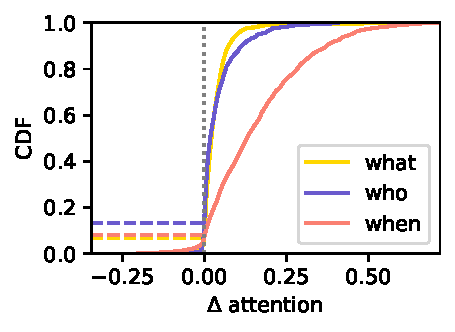
\includegraphics[width=1\textwidth]{Figures/attn_illustration_mistral.pdf} 
\end{minipage}
\caption{
(Right) CDF of $\Delta_{attn}$, the change of attention weight on the corresponding concept when asked the relevant question.%, on all 1,024 heads of Mistral-7B.
% For example, for ``when'', we compute $\Delta_{attn}$ as the attention weight on ``On July 20, 1969'' when asked the ``when'' question minus the average of the cases where the other two questions were asked.
%We then plot the CDF of such $\Delta_{attn}$ on all 1,024 heads of Mistral-7B.
In all cases, the attention significantly increases on the relevant tokens.% (p-value from one-sided t-test is at most 9e-90).
}
% \label{fig:attnillustration}
\end{figure}
\end{block}
%----------------------------------------------------------------------------------------

\begin{block}{Step 2: Head Selection}  
Even with the prompt, only a fraction of attention heads focus on the meaning of the response. 
We select the relevant head by computing the AUROC of each head on a validation set, and take the average attention of the top 10 heads.

\begin{figure}[ht]
\centering
% Text above the image
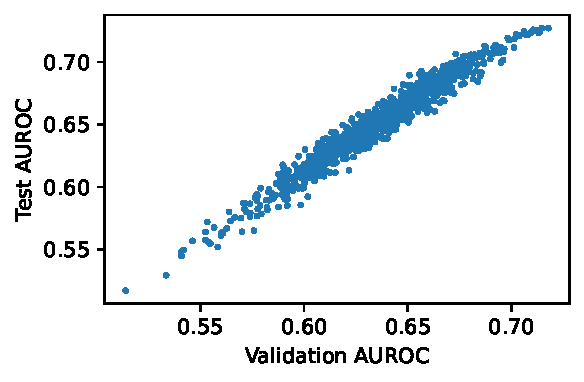
\includegraphics[width=0.42\textwidth]{Figures/head_consistency_mistral_nq_open_new.pdf} % Adjust 'width' as needed
% \vspace{-3mm}
\caption{
Test vs validation AUROC for $\ConfMethod$ using different heads' attention.%, on Natural Questions (\datasetnqopen) with Mistral-7B model. %~\citep{jiang2023mistral} model.
% accurcy measured by LLaMA2-70B
The ranking is highly consistent with a Spearman correlation of $>97\%$.
%We can thus pick only a small subset of the 1024 heads (or more for other LMs) to construct the final confidence measure $\ConfMethod$.
}
\label{fig:headvaltest}
% \vspace{-4mm}
\end{figure}

\textbf{\methodnameNext}:
While \methodnamePrompt already has very small overhead compared with running the LLM, one could further simplify it by dropping step 2 and reuse attention from the generation process.
This variant is referred to as \methodnameNext.
\end{block}
\end{column} % End of column 2.1

%----------------------------------------------------------------------------------------

\end{column} % End of column 2.2

%\end{columns} % End of the split of column 2

%\end{column} % End of the second column

\begin{column}{\sepwid}\end{column} % Empty spacer column

\begin{column}{\rightcolwid} % The third column



\begin{block}{\color{mydarkgreen}{Experiment Results}}


\textbf{Datasets}: CoQA (coqa), TriviaQA (trivia), Natural Questions (nq)

\textbf{Models}: LLaMA2 (13B), Mistral (7B), Gemma (7B)

\textbf{Evaluation Metrics}: 
\begin{itemize}
    \item AUROC ($\mathbf{1}\{{s_i\text{ correctly answers } x_i}\}\sim$ Confidence of $s_i$)
    \item AUARC: Area under the Accuracy-Rejection Curve. 
    The curve computes the accuracy at each rejection threshold (low confidence responses are rejected).
\end{itemize}


\begin{figure}[htbp]
  \centering
  \begin{minipage}[b]{0.99\textwidth}
    \centering
    \resizebox{\textwidth}{!}{%
      \begin{tabular}{c|ccccc|cc}
\toprule
AUROC & \baselineDegree(E) & \baselinePTrue & \baselineNLL & \baselineNLLNorm & \baselineSAR & \methodnamePrompt (Ours) & \methodnameNext (Ours) \\
\midrule
\datasettrivia(llama2) & 81.74$\pm$0.25 & 64.82$\pm$0.18 & 88.19$\pm$0.12 & 87.86$\pm$0.12 & 87.91$\pm$0.13 & \textbf{89.70$\pm$0.19} & \textbf{89.61$\pm$0.18}\\
\datasettrivia(gemma) & 84.00$\pm$0.19 & 81.82$\pm$0.18 & 88.72$\pm$0.11 & 88.11$\pm$0.08 & 88.09$\pm$0.08 & \textbf{89.71$\pm$0.14} & 89.42$\pm$0.11\\
\datasettrivia(mistral) & 81.85$\pm$0.30 & 68.78$\pm$0.28 & 88.81$\pm$0.15 & 88.64$\pm$0.14 & 88.74$\pm$0.13 & \textbf{90.76$\pm$0.18} & \textbf{90.73$\pm$0.15}\\
\datasetcoqa(llama2) & 69.93$\pm$0.57 & 53.64$\pm$0.41 & 69.50$\pm$0.40 & 72.59$\pm$0.44 & 72.78$\pm$0.47 & \textbf{73.34$\pm$0.74} & \textbf{73.36$\pm$0.57}\\
\datasetcoqa(gemma) & 70.03$\pm$0.68 & 55.99$\pm$0.42 & 70.83$\pm$0.46 & 71.96$\pm$0.57 & 72.38$\pm$0.55 & \textbf{73.30$\pm$0.57} & \textbf{73.64$\pm$0.63}\\
\datasetcoqa(mistral) & 69.84$\pm$0.52 & 52.33$\pm$0.42 & 68.97$\pm$0.38 & 70.60$\pm$0.38 & 70.87$\pm$0.41 & \textbf{71.79$\pm$0.75} & \textbf{71.91$\pm$0.63}\\
\datasetnqopen(llama2) & 71.61$\pm$0.51 & 52.51$\pm$0.47 & 66.57$\pm$0.33 & 69.48$\pm$0.50 & 70.43$\pm$0.46 & \textbf{73.73$\pm$0.49} & \textbf{73.54$\pm$0.46}\\
\datasetnqopen(gemma) & 73.32$\pm$0.68 & 63.66$\pm$0.46 & 72.09$\pm$0.65 & 75.81$\pm$0.65 & 75.88$\pm$0.68 & \textbf{77.95$\pm$0.58} & 77.17$\pm$0.65\\
\datasetnqopen(mistral) & 73.03$\pm$0.52 & 54.77$\pm$0.51 & 69.22$\pm$0.53 & 71.06$\pm$0.54 & 72.61$\pm$0.48 & \textbf{76.65$\pm$0.43} & 75.73$\pm$0.68\\
\bottomrule
\end{tabular}
    }
    \captionof{table}{AUROC of using confidence measures $\Conf$ to predict the accuracy of responses.
% Methods not significantly different from the best are in \textbf{bold}. % p=0.01
    }
    \label{tab:table1}
  \end{minipage}
  % \hfill
  % \begin{minipage}[b]{0.45\textwidth}
  %   \resizebox{\textwidth}{!}{%
  %     \includegraphics[width=\columnwidth]{pics/Efficiency.pdf}
  %   }
  %   \captionof{figure}{Computation time as a function of $N$. \datastructname gracefully handles large $N$, while BinarySearch does not finish.}
  % \end{minipage}
\end{figure}

Through transfer of the chosen attention heads, as well as case studies, we confirm that \methodname indeed picks up informative attention weights to weigh tokens.

\begin{figure}[htbp]
  \centering
  \begin{minipage}[b]{0.52\textwidth}
    \begin{table}%[ht]

\centering
%\begin{small}
   \resizebox{.9\columnwidth}{!}{
\begin{tabular}{c|ccc}
\toprule
 AUROC & \baselineNLLNorm & \methodnamePrompt & \methodnameNext\\
\midrule
\datasettrivia(llama2) & 87.86$\pm$0.12 & \textbf{88.59$\pm$0.85} & 88.37$\pm$0.87\\
\datasettrivia(gemma) & 88.11$\pm$0.08 & \textbf{89.03$\pm$0.61} & 87.43$\pm$0.94\\
\datasettrivia(mistral) & 88.64$\pm$0.14 & \textbf{89.70$\pm$1.43} & 88.46$\pm$1.93\\
\datasetnqopen(llama2) & 69.48$\pm$0.50 & \textbf{70.94$\pm$1.66} & 70.10$\pm$2.09\\
\datasetnqopen(gemma) & 75.81$\pm$0.65 & \textbf{77.21$\pm$1.06} & 74.99$\pm$1.30\\
\datasetnqopen(mistral) & \textbf{71.06$\pm$0.54} & \textbf{72.71$\pm$3.32} & \textbf{72.27$\pm$2.72}\\
\bottomrule
\end{tabular}
}\caption{
\textbf{The chosen heads are meaningful.}
We use heads chosen on \datasetcoqa, and apply to \datasetnqopen/\datasettrivia. 
Despite the big distribution shift, \methodname still outperforms vanilla sequence likelihood.
% AUROC using heads picked from \datasetcoqa.
% Despite the big distribution shift from \datasetcoqa to \datasetnqopen/\datasettrivia, the heads chosen on \datasetcoqa still provides attention weights that significantly improves the AUROC.
}
\label{table:main:exp:roc:coqa_transfer}
\end{table}
  \end{minipage}\hfill
  \begin{minipage}[b]{0.45\textwidth}
      \begin{figure}[ht]
\begin{small}
% \resizebox{.9\columnwidth}{
  \begin{framed}
  \raggedright
\textit{Q1:} how early did he want to get there?\\
\textit{R1:} \attnplus{an hour before} the time\\
\textit{Q2:} What does Barwell think of him?\\
\textit{R2:} \attnplus{he} is \attnplus{not fit} to be his guard\attnplus{ian}\\
\textit{Q3:} who is Susan Boyle?\\
\textit{R3:} \attnplus{Susan} Bo\attnplus{yle is a Scottish singer who} became \attnplus{famous} after appearing on the TV show "Britain\attnplus{'}s Got Talent" in \attnplus{2}009\attnplus{.}
  \end{framed}
% }
  \end{small}
\caption{
Tokens whose attention is increased are \attnplus{marked} (others decreased).
As expected, such re-weighting are not always interpretable, but help locating the more relevant tokens in general.
}\label{fig:main:case}
\end{figure}
  \end{minipage}
\end{figure}


\end{block}

%----------------------------------------------------------------------------------------
%	REFERENCES
%----------------------------------------------------------------------------------------

%\begin{block}{References}

%\nocite{*} % Insert publications even if they are not cited in the poster
%\small{\bibliographystyle{unsrt}
%\bibliography{new_poster}\vspace{0.75in}}

%\end{block}

%----------------------------------------------------------------------------------------
%	ACKNOWLEDGEMENTS
%----------------------------------------------------------------------------------------

\setbeamercolor{block title}{fg=red,bg=white} % Change the block title color

\begin{block}{Acknowledgements}

\small{\rmfamily{This work was supported by NSF award SCH-2205289, DMS-1439786, SCH-2014438, IIS-1838042, NIH award R01 1R01NS107291-01.}} \\

\end{block}

%----------------------------------------------------------------------------------------
%	CONTACT INFORMATION
%----------------------------------------------------------------------------------------

\setbeamercolor{block alerted title}{fg=black,bg=norange} % Change the alert block title colors
\setbeamercolor{block alerted body}{fg=black,bg=white} % Change the alert block body colors

\begin{alertblock}{Additional Information}

\begin{itemize}
\item Code: \href{https://github.com/zlin7/FavMac}{https://github.com/zlin7/ContextSL}
\item Email: \href{mailto:zhenlin4@illinois.edu}{zhenlin4uiuc@gmail.com}
\end{itemize}

\end{alertblock}

%----------------------------------------------------------------------------------------

\end{column} % End of the third column

\end{columns} % End of all the columns in the posterf

\end{frame} % End of the enclosing frame

\end{document}
